% --------------------------------------------------------------------------------------
%                   LATEX TEMPLATE FOR DISSERTATION (HONS)
% --------------------------------------------------------------------------------------
\documentclass[11pt]{book}

\usepackage{amsfonts, amsmath, amssymb}  
\usepackage{times}

%\usepackage[backref=page,pagebackref=true,linkcolor = blue,citecolor = red]{hyperref}
%\usepackage[backref=page]{backref}

\usepackage{graphicx}
\DeclareGraphicsExtensions{.pdf,.png,.jpg}

\setlength{\oddsidemargin}{1.5cm}
\setlength{\evensidemargin}{0cm}
\setlength{\topmargin}{1mm}
\setlength{\headheight}{1.36cm}
\setlength{\headsep}{1.00cm}
%\setlength{\textheight}{20.84cm}
\setlength{\textheight}{19cm}
\setlength{\textwidth}{14.5cm}
\setlength{\marginparsep}{1mm}
\setlength{\marginparwidth}{3cm}
\setlength{\footskip}{2.36cm}

\newcommand{\code}[1]{\texttt{#1}}
\newcommand{\pkg}[1]{\textsf{ \bf #1}}
\newcommand{\R}{\textsf{R}}



\begin{document}
\pagestyle{empty}

%: ----------------------------------------------------------------------
%:                  TITLE PAGE: name, degree,..
% ----------------------------------------------------------------------

\begin{center}

\vspace{1cm}

%%% Type the thesis title below%%%%%%%%%%%%%%%%
{\Huge         High-Performance Hadoop Map/Reduce R Interface Enhancement}

\vspace{25mm} 


\includegraphics[width=3.5cm]{logo}

 \vspace{35mm}

%%%%%Type Your Name Below%%%%%%%%%%%%
{\Large       Noah Zhang}

	\vspace{1ex}

Department of Statistics

The University of Auckland

	\vspace{5ex}

 %%%%%Typing Your Supervisors Name Below%%%%%%%%%%%%
Supervisor:             Simon Urbanek

	\vspace{30mm}

A dissertation submitted in partial fulfillment of the requirements for the degree of BSc(Hons) in Statistics, The University of Auckland, 2020.

\end{center}

\newpage


%: --------------------------------------------------------------
%:                  FRONT MATTER:  abstract,..
% --------------------------------------------------------------
\chapter*{Abstract}       
\setcounter{page}{1}
\pagestyle{headings}
% \pagenumbering{roman}

\addcontentsline{toc}{chapter}{Abstract}


 Put your abstract  here.  The abstract should contain a brief summary of the aim, methodologies, 
finding and conclusions of the dissertation.  The abstract should normally be fewer than 350 words.


One of the most widely used parallel programming models today is MapReduce. MapReduce is easy both to learn and use, and is especially useful in analyzing large datasets. While it is not suitable for several classes of scientific computing operations that are better served by message-passing interface or OpenMP, such as numerical linear algebra or finite element and finite difference computations, MapReduce's utility in workflows frequently called “big data” has made it a mainstay in high performance computing. This chapter introduces the MapReduce programming model and the Hadoop open-source framework which supports it.

Big data is concern massive amount, complex, growing data set from multiple autonomous sources. It has to deal with large
and complex dataset that can be structured, semi-structured or unstructured and will typically not fit into memory to be processed.
MapReduce is a programming model for processing large datasets distributed on a large clusters.A rapid growth of data in recent time,
Industries and academia required an intelligent data analysis tool that would be helpful to satisfy the need to analysis a large amount of
data. MapReduce framework is basically designed to compute data demanding applications to support effective decision making. Since
its introduction, remarkable research efforts have been put to make it more familiar to the users subsequently utilized to support the
execution of enormous data intensive applications. This survey paper highlights and investigates various applications using recent
MapReduce models.





%: --------------------------------------------------------------
%:                  END:  abstract
% --------------------------------------------------------------


%: ----------------------- contents ------------------------
\setcounter{secnumdepth}{3} % organisational level that receives a numbers
\setcounter{tocdepth}{3}    % print table of contents for level 3
\tableofcontents            % print the table of contents
% levels are: 0 - chapter, 1 - section, 2 - subsection, 3 - subsection

%: --------------------------------------------------------------
%:                  MAIN DOCUMENT SECTION
% --------------------------------------------------------------
	
\chapter{Introduction}%    \chapter{}  = level 1, top level

A thesis should always have an introduction.  The purpose is to describe the general subject area, state the research problem of interest, outline the main results of the thesis, and put the results in context with the wider subject area and its applications.

The main body of the text must be divided into a logical scheme which  is followed consistently throughout the work.  
 It usually starts with an introduction chapter  and ends with  a conclusion chapter. See, for example, the table of contents on page 3. 

There is strict  35-page limit  for an applied mathematics dissertation,  including  the references  but excluding  appendices. 

\chapter{Concept of Big Data}

Big data concerns huge amounts, complex and diverse sets of information that is growing at ever-increasing rates. The size of the data suggest that we will need to deviate from the traditional processing methodologies and to adapt an inexpensive and efficient way through distributed/parallel computing.\\

Today, we can find upwards of 800 million webpages providing documentation on big data. Enthusiasts believe that Big Data is the next big thing after Cloud [1]. 

\section{Characteristics of Big Data}

The concept of big data is generally vague without a formal definition, however the general consensus is that there are specific attributes that define big data The four characteristics of big data are Volume, Velocity, Variety and Veracity [2]. 

\begin{center}
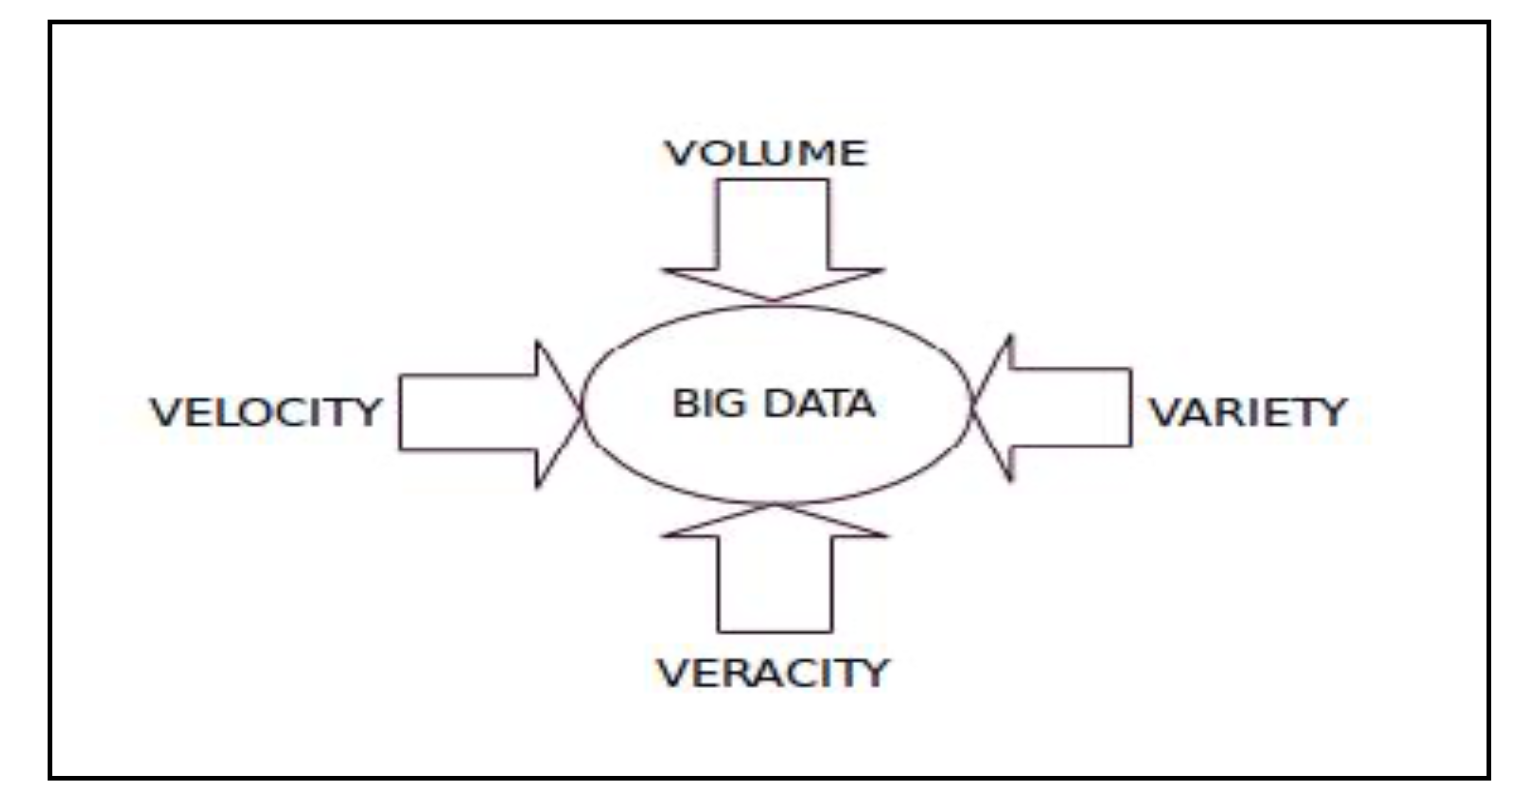
\includegraphics[width=10cm]{4vbd}\\
\end{center}

The main characteristic that makes data “big” is its sheer volume. According to estimates by IBM, we can expect at least 40 Zettabytes (43 Trillion Gigabytes) of data to be created in 2020 [3]. The volume of data sets being processed and analysed has reached sizes larger than terabytes and even petabytes. This suggests that data sets these days are becoming too large to process within a single desktop machine/processor. \\

Velocity is the speed at which data is generated. High velocity data is generated with such a pace that it may require certain distributed processing techniques. Good examples of high velocity data includes social media posts.\\

Variety is the source of the data which can be found in different forms such as text, numerical, images, audio and video records. The variety in the data will require distinct processing capabilities or algorithms to handle different formats. \\

Veracity is the quality of the data. Information may be volatile or incomplete seen in low veracity data sets containing a high percentage of meaningless data referred to as noise. On the other hand, high veracity data hold records that are valuable to analyse and contribute in a meaningful way to the overall results.

\section{Structure of Big Data} 

Big data can be categorised as structured or unstructured.\\
 
Structured data is usually stored and managed in relational databases with predefined data models. Examples of relational database applications with structured data include customer information, sales transactions, airline reservations systems, and billing systems. This type of structured data within relational databases can be accessed using Structured Query language (SQL).\\
 
Unstructured data, in contrast, has its internal structure but it is not structured through pre-defined data models or schema. As it may comes in many different formats, it cannot be stored in relational databases which also becomes a real challenge for systems to process and analyse. The unstructured data may be stored within non-relational databases like NoSQL.

\chapter{MapReduce Framework}

At present, with data being generated at an exponential rate, there is the need to deploy data intensive application and storage clusters in order to keep up with the amount of data. To handle such problem, Google developed the MapReduce programming model for distributed computing based on the Java language [5].

\section{Concept of MapReduce}

There are multiple approaches for processing relatively smaller datasets, however larger datasets require a different approach specifically for data that is too big to fit in memory. The traditional approach to process data on a single machine is to break data into individual chunks which is then loaded and processed sequentially on the machine. 

MapReduce is a processing technique/programming model for distributed computing based on Java. It is designed to process large datasets using the same splitting approach by breaking down the dataset into independent chunks. But instead of processing the chunks sequentially, the chunks are processed in parallel on a collective group of computers known as a cluster. The results of the individual chunks are then aggregated and returned as output.\\


\includegraphics[width=8cm]{keyvalue} \\

The algorithm operates on key-value pairs, which means that it takes a set of input key-value pairs and produces a set of output key-value pairs. In addition, the user is required to specify two functions for the Mapper and Reducer. The Mapper takes the input and produce the intermediate key-value pairs which is passed to the Reducer to create a set of output key-value pairs. The Reducer combines all the values associated with each key to create a smaller set of values. This enables us to input data that may be too large to fit in standard memory.\\

In the simplest form of the MapReduce model, the user only specifies the Map function. In this case, the output will consist of the intermediate key-value pairs which is ordered by the keys. 

{\bf TEST: 
See also Section~\ref{sec:mapreduce}. }

\section{The MapReduce Process}
\label{sec:mapreduce}

The complete process typically consists of four operations namely, splitting, mapping, shuffling and reducing.\\

1. Splitting - the process whereby larger data sets are split into smaller data sets based on the block size. The default size of each block is 64MB, however this can be adjusted by the user. The number of mappers will depend on the number of blocks generated by the split, i.e. if there are 3 blocks then there will only be 3 mappers.\\

2. Mapping - the purpose of the mapper is to process the input data. In this phase, data in each chunk is passed to a user specified map function and returns output in the form of key-value pairs. For example, if a file contains 100 blocks to be processed, you can have 100 mappers which can run together to process one block each or have 50 mappers running together to process two blocks each. The Hadoop framework decides how many mappers to allocate based on the size of the data and the memory block available on each mapper server.\\

3. Shuffling - the process by which data from the mappers is transferred to the reducers known as the intermediate values. The data from all mappers are sorted by the key, split among the reducers and sorted by the key. Without this step, there will be no input for the reducer.

4. Reducing - the reducer is guaranteed to have all records associated with each key. In this phase, the key-value output from the shuffling stage are aggregated.  It is important to note that one key can only be in one reducer, else the aggregation will be non-functional. In other words, this operation is a summary of the complete dataset. 

obtains the intermediate values, sorted by the key. The value list contains all values with the same key produced by mappers. Each reducer emits zero, one or multiple output key/value pairs for each input key/value pair.


\section{Examples}



\section{Advantages of MapReduce}

The main advantage of MapReduce is that it is highly scalable. This is due to the ability to process large data sets across multiple computer nodes. These servers can be inexpensive and can also operate in parallel. This simple scalability is what attracts many users to utilise the MapReduce model.

Other advantages include cost efficiency, security and authentication, parallel processing, availability, resilient and simple.


\chapter{The Hadoop Framework}

Hadoop is Apache's free and open-source implementation of the MapReduce framework. Apache Hadoop offers reliable, scalable, parallel and distributed computing scaling up from a single server to a network of multiple computers[4]. It was developed with the purpose of having a data store that allow organisations to leverage big data analytics with cost efficiency in mind.\\

%There are two main components of the Hadoop Framework: Storage and Processing

\section{Hadoop Architecture}

Hadoop follows a master/slave architecture design for data storage and distributed data processing using HDFS and MapReduce respectively. The master node for data storage is NameNode while the master node for parallel processing is the Job Tracker. The slave nodes are comprised of other machines in the Hadoop cluster which stores the data and performs the computations. Each slave node have a DataNode and a TaskTracker that synchronises the process respectively. \\

\begin{center}
 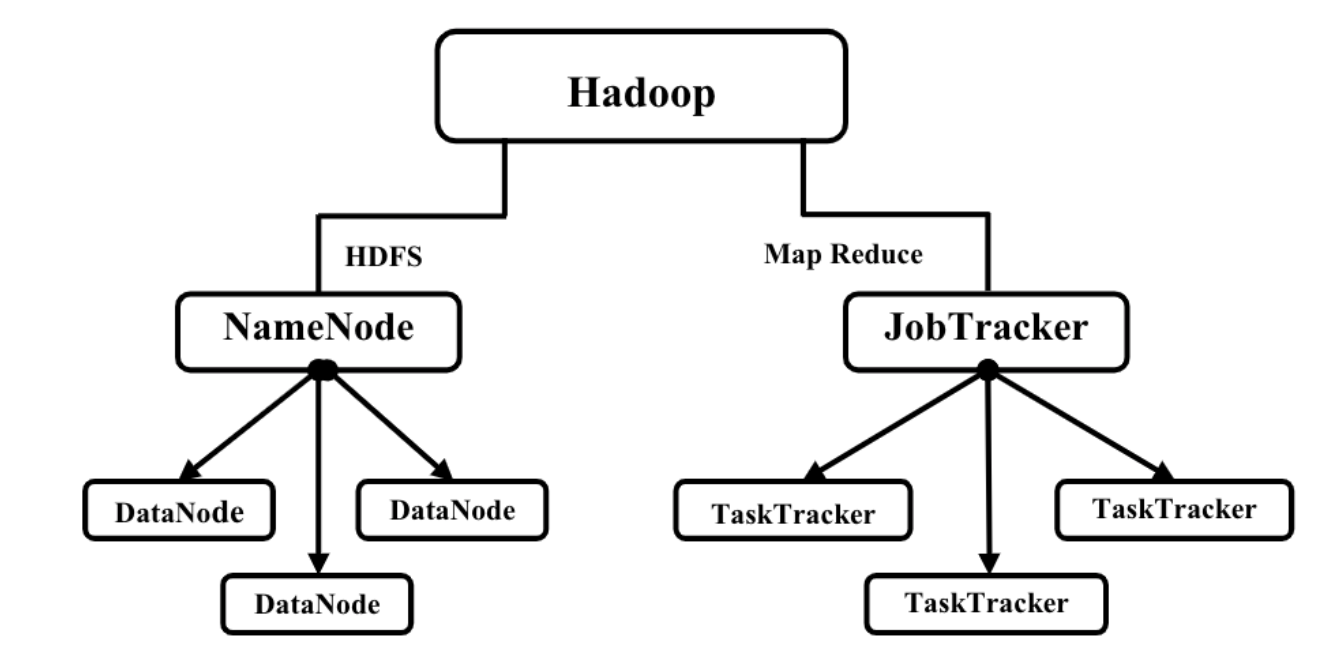
\includegraphics[width=10cm]{hadoop}\\
 \end{center}

The Hadoop system can be set up via cloud or locally. The cluster we will be running is a set up of 8 virtual machines.

\section{Storage - HDFS}

The storage component of the Hadoop architecture is known as the Hadoop Distributed File System (HDFS). The NameNode runs on the master node and manages metadata about the file system in a file named fsimage. This metadata is cached in main memory to provide faster access to the clients on read/write requests. The NameNode controls also manages the slaves by splitting files into chunks (default 64 megabytes) and distributing them across each DataNode in the cluster. The DataNodes are primary storage elements of HDFS where chunks of data are stored and replicated according to the instructions from the NameNode. Secondary NameNode is to periodically read the file system, log changes and applying them to the fsimage file. This will enable the NameNode to boot faster.\\

The main advantages of HDFS is data locality and fault tolerance. Data locality allow the nodes to manipulate the data they have access to which results in faster and more efficient processing while handling faults through the process of replicating files across each slave node[4].\\

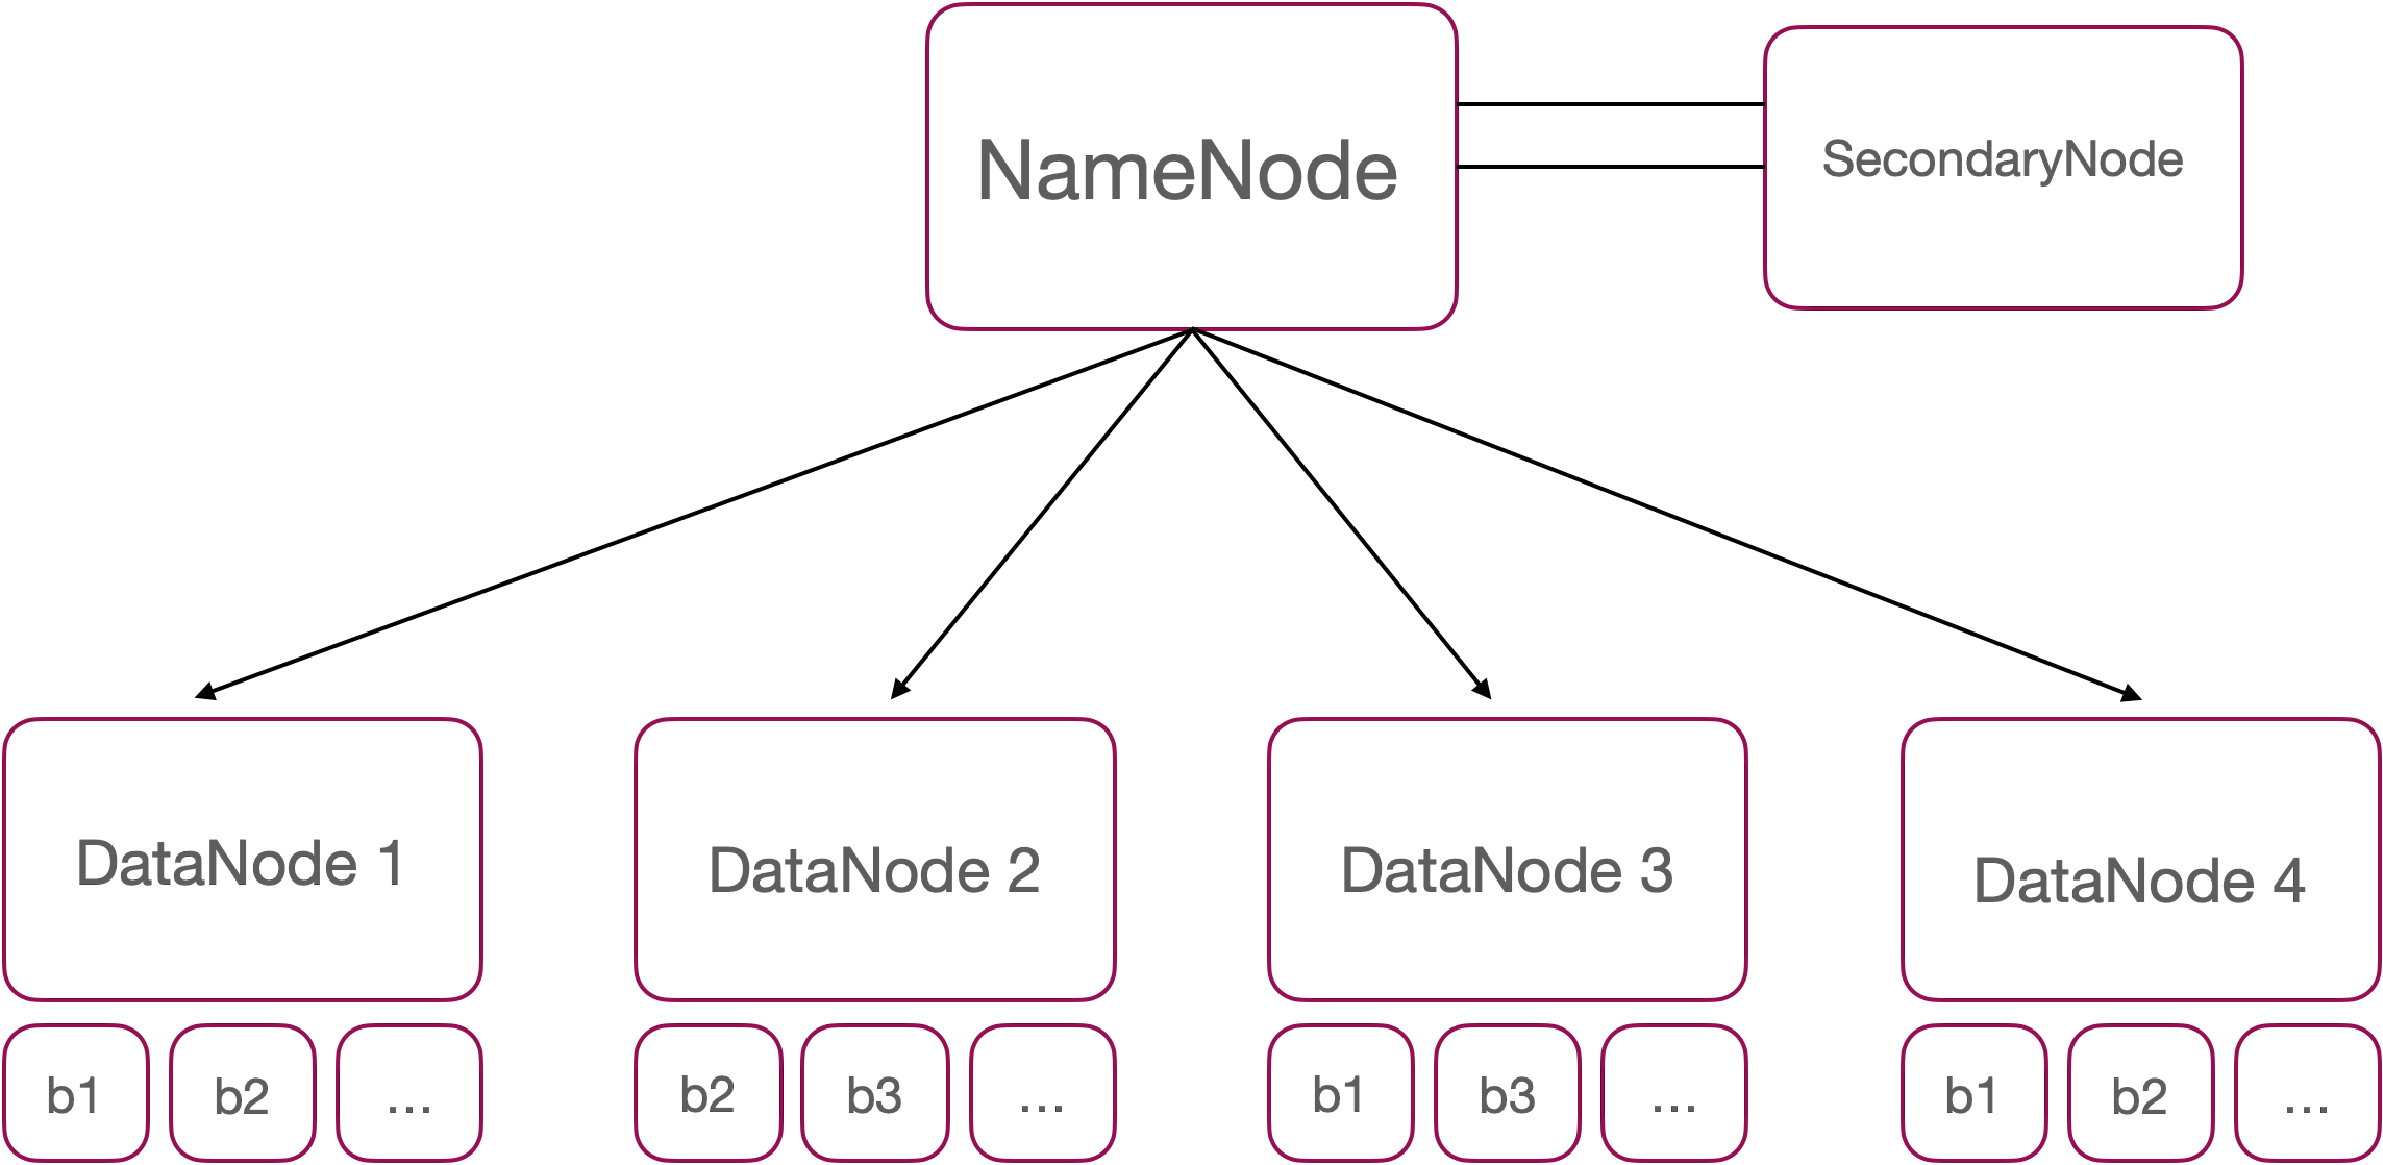
\includegraphics[width=8cm]{hdfs}

\section{Processing - MapReduce}

In a MapReduce job, the input is broken down into multiple chunks which are processed by the map phase and then the output of the map phase is passed as input to the reduce phase. The input and output files are stored in the file system, while the output of the map phase (known as intermediate results) are only stored temporarily in the process. As the process runs in parallel, the reduce task on specific nodes may begin once its map tasks is complete rather than waiting on all map tasks to complete.\\

Similar to HDFS, the MapReduce process also utilises the master/slave architecture in which the JobTracker runs on the master node while the TaskTracker runs on each slave node. \\

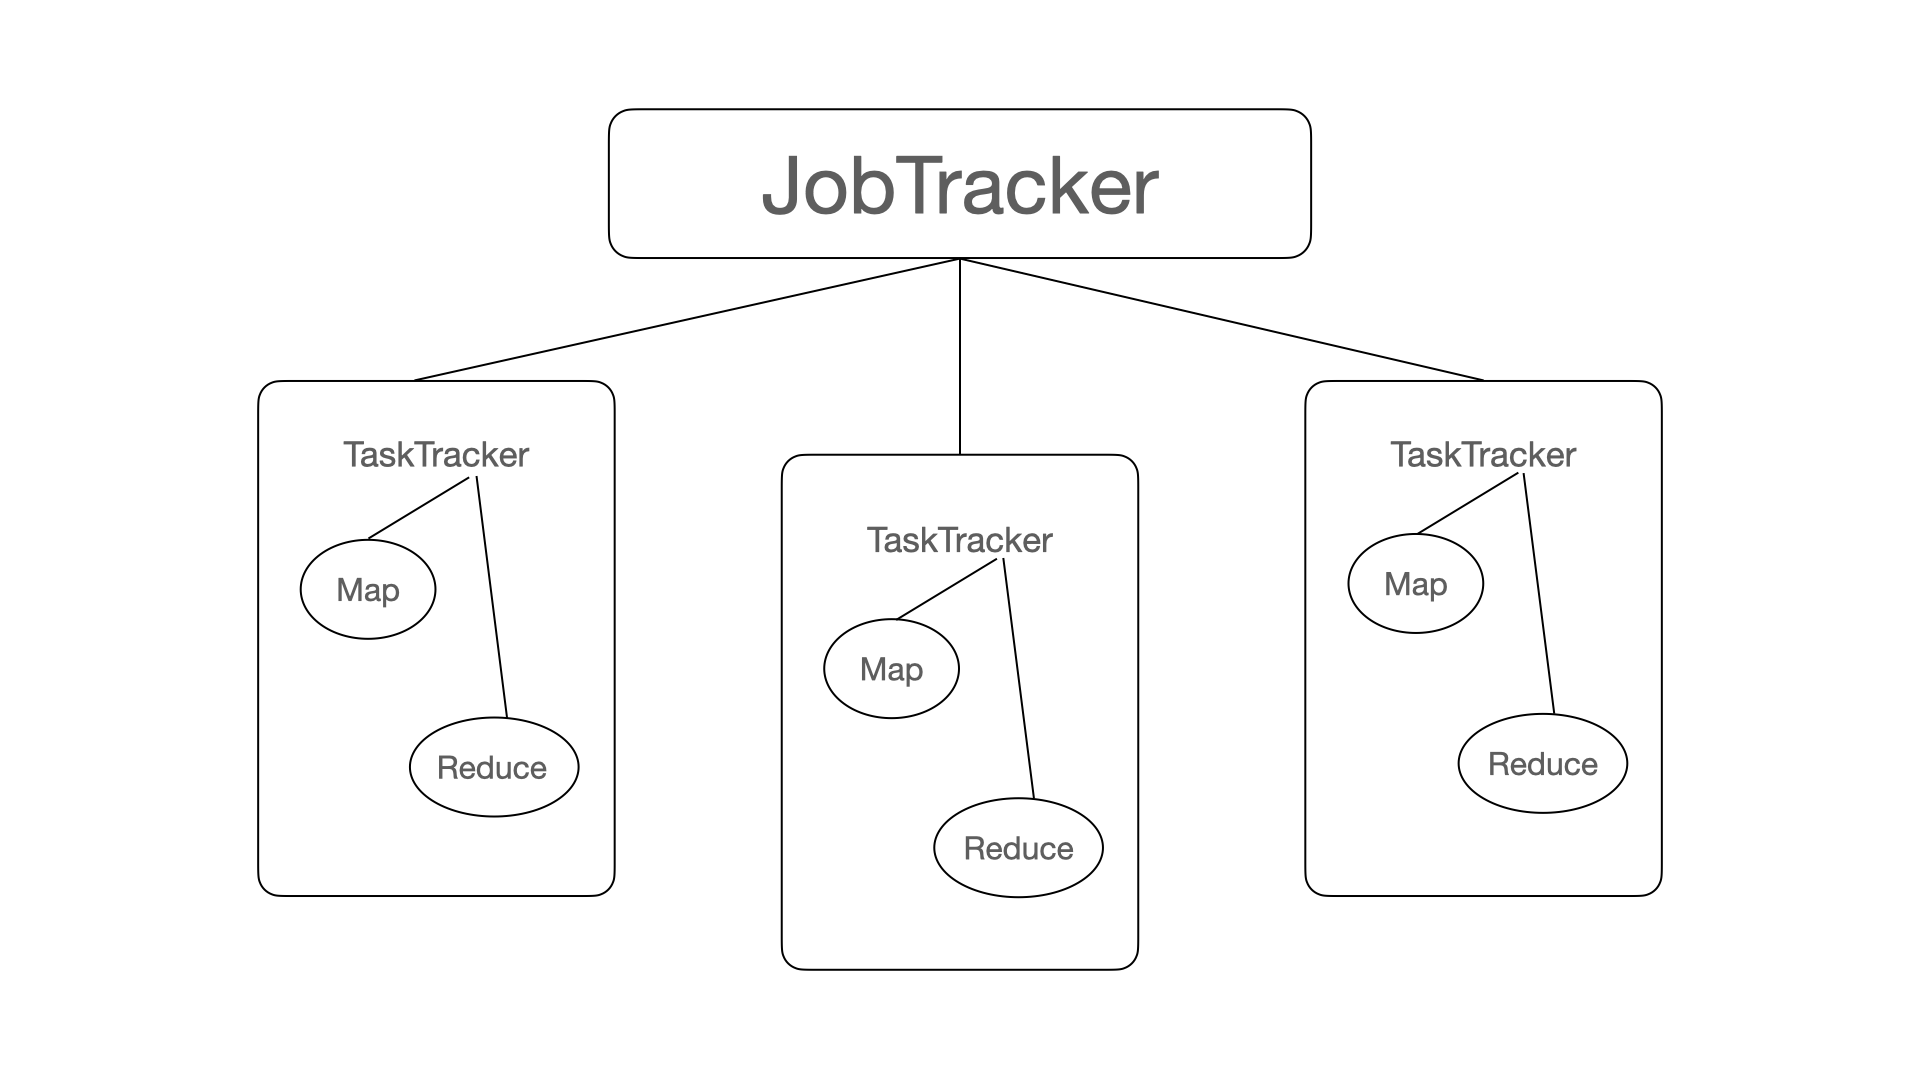
\includegraphics[width=8cm]{jobtracker}

The JobTracker monitors the MapReduce tasks carried out by the TaskTracker running on the slave nodes. The user will only interact with the master node by submitting jobs to the JobTracker. The JobTracker then locates and submits the jobs to the TaskTracker. The slave nodes are monitored by the JobTracker through heartbeat signals to determine whether a node has failed. The JobTracker is a point of failure for the Hadoop MapReduce service and if it goes down, all jobs will be stopped. \\

The TaskTracker runs on the slave nodes in a cluster and receives jobs from the JobTracker to execute the MapReduce tasks. Each TaskTracker has an allocation of task slots which indicate the number of tasks it can accept. The JobTracker will delegate jobs to the TaskTracker based on the number of available/empty slots while the TaskTracker will periodically send heartbeat signals to inform the JobTracker of any issues. TaskTracker failure is not considered fatal as tasks can be reallocated to another node when it becomes unresponsive.\\

\chapter{Hadoop Streaming}

Hadoop streaming is a utility that comes with the Hadoop distribution which allow users to create and run MapReduce jobs to be executed in the Hadoop cluster using other languages. By default the Hadoop MapReduce framework is written in Java but it utilizes Unix streams to pipe between Hadoop and our MapReduce program so we can use any language which can read standard input and write to standard output for our MapReduce program. MapReduce programs can be written in mutiple languages such as R, Python, Perl, PHP, C++, etc. The utility is packed in a JAR file. 

\section{Purpose}

Using the utility, we can create executable scripts to run MapReduce Jobs. Furthermore, we can create executable scripts to run the mapper and reducer functions which are passed to Hadoop streaming. The utility creates map and reduce jobs and submits them to the cluster which can then be monitored, thus enabling a person to write MapReduce job in the language of their choice without having any knowledge of Java.

\section{Syntax}

The syntax below can be used to run MapReduce jobs written in a different language to process data using the Hadoop MapReduce framework.\\

\begin{verbatim}
$HADOOP_HOME/bin/hadoop jar $HADOOP_HOME/hadoop-streaming.jar 
    -input myInputDirs 
    -output myOutputDir 
    -mapper /bin/cat 
    -reducer /usr/bin/wc
\end{verbatim}

The input command is used to provide the directory fo the input which the output command is used to provide the output directory. The mapper command is used to specify the executable mapper class while the reducer command is used to specify the executable reducer class.

The mapper command is used to specify the executable mapper class while the reducer command is used to specify the executable reducer class.

\section{How it Works}

Let us now explore how Hadoop streaming works.\\


\includegraphics[width=14cm]{streaming}\\

The mapper and reducer are scripts/functions created by the user that reads in the input line by line from standard input and returns the output to standard output. If the mapper script/function is specified, the mapper will converts the inputs into lines and converts the lines to the standard input which feeds into the mapper. In the process, the mapper converts each line into a key and value pair returned as standard output. If the reducer script/function is specified, the reducer then draws the line-oriented key value pairs from the mapper as standard input and converts each line collected into a key/value pair. This is then emitted to standard output. 

For both the mapper and the reducer, first entry of the line is the key followed by the value which is separate by a tab character. If there is no tab character in the line, then the entire line is considered as the key and the value is considered null. 

\section{Advantages}

\begin{enumerate}
\item Availability - the utility comes with the Hadoop distribution hence does not require further installation of softwares.
\item Learning - relatively easy to learn as it requires basic unix coding.
\item Reduce Development Time - it is much quicker to write mapper and reducer scripts/functions whereas using native Java MapReduce application is more complex as it requires the application to be complied, packaged, and exporting the JAR file.
\item Faster Conversion - it takes very little time to convert data from one format to another using Hadoop streaming especially when the input and output formats are specified.
\item Testing - input and output data can be tested quickly by using it with Unix or command line tools.
\end{enumerate}

\chapter{HMR Hadoop MapReduce Package for R}

HMR is a package developed in R which acts as an interface which give R users the ability to execute Hadoop Map/Reduce jobs. It is highly efficient as it utilise chunk-wise processing as well as automated conversion to and from R objects. This allows users to feed existing R code to Hadoop with ease. There are other packages in R which uses the traditional key-value operations such as the \pkg{rmr2} package.

\section{Examples}

Using the current package, we will perform some simple calculations using the taxi data set store in HDFS. We can access the files through Unix shell and simple Bash commands.

\begin{verbatim}
hadoop@hdp:~$ hadoop fs -ls taxi
\end{verbatim}

This data set contains 19 attributes ranging from vendor ID, pickup/drop off times, distance, location, payment, number of passengers, etc. \\

The following R script streams the MapReduce process through the HMR function in R. The script will calculates the number of lines/records for January 2015. with the map function being the shell command for counting the number of lines. The script uses the default formatter as no formatters have been specified.

\begin{verbatim}
hmr(hinput("taxi/2015/01"), map="wc -l", reducers=0, wait=FALSE)
\end{verbatim}

The following R script also performs the same line count calculation. However, the formatter has been specified which only include the first 5 fields of the data set. Instead of using shell command as the previous script, the mapper is using a R function "nrow" which also calculates the numbers of rows.
 
\begin{verbatim}
hmr(hinput("taxi/2015/01",
           formatter=function(o) dstrsplit(o, list(vendor=1, NA, NA, 
           	pass=1, dist=1), sep=",", strict=FALSE)),
    map=function(d) nrow(d), reducers=0, wait=FALSE)
\end{verbatim}

\section{Concept of HMR Package in R}

The HMR package is essentially a Hadoop streaming API which runs in R. This allows the user to run MapReduce jobs and write formatter functions in R as opposed to writing scripts in the native language Java. The idea is stream the data from a file path/connection in Hadoop and parse into R as individual blocks represented in raw binary format. The data is converted into R objects such as matrix/data frames which enables the user to write the formatter functions. The functions is written in the R language for the mapper and reducer to process each of the blocks simultaneously. The final script is converted to Java and passed to Hadoop to execute the MapProduce job. The output is converted back to raw bytes and stored as HDFS which can be access through Hadoop.

\section{Current Approach}

In order for us to execute MapReduce jobs, we will require a server/cluster with Hadoop set up. The file path/connection defines the HDFS file path and input source. The input is read into R using chunk.reader from \pkg{iotools}. HMR can take two types of input objects: \code{hpath} and \code{hinput}. Hpath only contains the path of the input whereas hinput has an additional formatter argument which allows the user to specify the class of the input variables as a vector or a list. This will require the user to have some familiarity or knowledge of structure of the data. 

The current logic allows the user to specify the function for both the mapper and reducer as a list or either one of the map or reduce function as a vector. If no list or vector is specified for the formatter, then HMR defaults to the default formatter which uses the mstrsplit function with tab as the key separator and $\mid$ as the the column separator. With the default formatter, the class of the variables are in the string/character format which is highly inefficient. If separate formatters are required, the formatter can be a list with the entries map and/or reduce specifying the corresponding formatter function. 

\section{Leveraging\pkg{iotools} for Efficiency}

HMR is highly efficient as it leverages the \pkg{iotools} package in \R. It is a set of tools for quickly importing and processing datasets using any data source. The functions packaged in \pkg{iotools} are comparatively faster than the native functions in R as well as other packages such as bigmemory, readr, foreach, etc. 

The two functions chunk.reader and read.chunk are functions used in the HMR package. chunk.reader essentially converts a binary connection into chunks stored as an object in R while preserving the integrity of the lines. On the other hand, chunk.read converts this object into a raw vector for each subsequent chunk. The efficiency comes from the use of binary data and raw objects in R which allow fast chunk-wise processing. 

Other core functions in the \pkg{iotools} package used in the HMR package are \code{mstrsplit} and \code{dstrsplit}. It takes either a raw or character vector and splits it into a matrix or data frame in R with the specified separator. These functions are able to minimize the copying of data and avoid the use of intermediate strings to improve performance.

%%%% talk about as.output, reverse of dstrsplit/mstrplit

\chapter{Package Enhancement - Automating Formatters}

The motivation behind this project is to infer the input formatters for the mappers and the reducer by automatically detecting the class of the attributes from the input. 

We know the importance of formatters with regards to writing the map and the reduce functions to execute the MapReduce job. Currently there is no way to infer the formatter for the reducer, hence it is particularly difficult to write the reduce function. Writing the formatter for the mapper is relatively easy as we can access the input data with ease, but it is not the same case for the reducer unless we know the output of the mapper.

The current approach allows the user to specify the formatter for the mapper and the reducer or the package defaults to the default formatter which is highly inefficient as it reads the variables as strings/characters. This may lead to running additional MapReduce jobs in order to reach the final desired output. It also adds more coding to the reducer function in the case where the data type may needs to be converted appropriately for the reducer to run successfully.

%%%The issue with the default formatter is that it is highly inefficient to read in data as string/characters. It will also require additional coding in the map and reduce functions to convert the data types in order to run the job.

%gives user customisation

\section{Concept of Auto Detection}

The idea is to take a sample of the complete data set and use that to automatically detect the formatters for the mapper. The easiest way is to take the first megabyte or specified number of lines to perform the detection. The drawback with this approach is that we have to assume the data types will be consistent across the complete data set. 

After we have the subset in the form of raw bytes, we convert it into a matrix separated by each variable of the data set. In the matrix form, we can detect the data type in each column as logical, integer, numeric, complex, character or factor. It should return a vector of the data type for each variable based on each column of the matrix. 

\section{New Approach - Two Approaches}

%talk about the idea of running in dynamic and in advance

The enhancement provides automatic detection of the formatter for the mapper and the reducer in the absence of user specified formatters. The additional argument included in the HMR function is "autoformatter" which is set to TRUE for dynamic detection, FALSE for static approach and defaults to NULL if the user wish to specify their own formatters.

There are two approaches for detecting the formatter. The original approach is to detect the formatter in advance which we refer to as the "static" approach. The alternative approach is to run the on each chunk during the MapReduce process. This is referred to the "dynamic" approach.

\subsection{Dynamic Approach}

With the dynamic approach, it is a lot simpler to detect as we already have the data available in raw bytes so all we need to do is to find the data types for the formatter. We can simply detect both the formatter for the mapper and the reducer using the same function as it runs within the process. 

The function named "coltypes" which takes the data in raw bytes, the specified column separator, the row name separator, specified number of lines, and the header. Using the mstrsplit function from\pkg{iotools} and the specified arguments, we can convert the raw data into matrix object in R. With each column of the matrix, we can apply the functions type.convert to create the appropriate data object across the rows and call the class function to determine the object class of each column/attribute. Using matrix operation functions we can operate on each of the columns and returns a vector containing the data type for each variable in the data set.

advantages: each chunk may vary, 
disadvantage: no header

\begin{verbatim}
  ## dynamic approach
  coltypes <- function(r, sep=formsep, nsep='\t', 
                       nrowsClasses=25L, chunksize=size, header=TRUE) {
    if (sum(r==10) < nrowsClasses) {
      nrowsClasses = sum(r==10)
      r <- r[1:chunksize]
      r <- r[1:tail(which(r==10),1)]
    }
    subset = mstrsplit(r, sep=sep, nsep=nsep, 
    			nrows=nrowsClasses, skip=header)
    colClasses = apply(subset, 2, function(x) 
    				class(type.convert(x, as.is=TRUE)))
    if (header) {
      col_names = mstrsplit(r, sep=sep, nsep=nsep, nrows=1)
      if ((length(col_names) - 1 == length(colClasses)) && !is.na(nsep))
        col_names = col_names[-1]
      names(colClasses) = col_names
    }
    colClasses
  }
\end{verbatim}

\subsection{Static Approach}

The static approach detects the formatter ahead of the time prior to executing the MapReduce job. As we are using a subset of the complete data set in advance, we will need to create a pipe to the HDFS location and read in the specified size of the sample data to perform the detection of the formatters. Using chunk.reader and chunk.read from \pkg{iotools} we can read in the connection and convert to a raw vector as input for the mapper. With the raw vector, we can leverage the coltypes function from the dynamic approach to detect the formatter for the mapper.

The challenge for this approach is that we have to obtain the intermediate key-value pairs in order to automatically detect the formatter for the reducer. Hence there is an extra step which is to execute the mapper first using the subset to generate the mapper output that we will feed into the reducer as input. As the output of the mapper is an R object, we will need to convert it back to a raw vector using as.output from the \pkg{iotools} package. From here we can use the same coltypes function to detect the formatter for the reducer. The output from the detection will be a vector containing the data type for each variable in the data set.


The risk with this approach is data may be incomplete, i.e. may be logical due to missing values. More suitable for known structure.

\begin{verbatim}
  ## new static approach
  guess <- function(path, chunksize=size, header=TRUE, map) {
    f <- pipe(paste("hadoop fs -cat", shQuote(path)), "rb")
    cr <- chunk.reader(f)
    r <- read.chunk(cr, chunksize)
    colClasses = coltypes(r)
    close(f)
    if (!missing(map)) {
      m = map(dstrsplit(r, colClasses, sep=formsep, skip=header))
      c = coltypes(as.output(m), header=FALSE)
      if (length(c) == length(names(m)))
        names(c) = names(m)
      rm(list=c("cr", "r", "f"))
      list(map=function(x) dstrsplit(x, colClasses, 
      	sep=formsep, skip=header), 
           reduce=function(x) dstrsplit(x, c, sep="|", 
           	nsep="\t", skip=FALSE))
    }
    else function(x) dstrsplit(x, colClasses, sep=formsep, skip=header)
  }
  \end{verbatim}

\section{Formatter Logic}

\begin{verbatim}
  ## formatter logic
  map.formatter <- NULL
  red.formatter <- NULL
  if (!missing(formatter)) {
    if (is.list(formatter)) {
      map.formatter <- formatter$map
      red.formatter <- formatter$reduce
    } 
    else map.formatter <- red.formatter <- formatter
  }
  else {
    if (missing(autoformatter)) {
      if (inherits(input, "hinput"))
        map.formatter <- attr(input, "formatter")
      if (is.null(map.formatter)) map.formatter <- .default.formatter
      if (is.null(red.formatter)) red.formatter <- .default.formatter
    }
    else {
      if (isTRUE(autoformatter)) {
        map.formatter <- function(x) dstrsplit(x, coltypes(x), 
        	sep=formsep, skip=TRUE)
        if (!missing(reduce)) 
          red.formatter <- function(x) dstrsplit(x, 
          	coltypes(x, header=FALSE), nsep='\t')
      }
      else if (autoformatter==FALSE) {
        if (!missing(reduce)) {
          formatter <- guess(paste0(input,"/*"), map=map)
          map.formatter <- formatter$map
          red.formatter <- formatter$reduce
        }
        else map.formatter <- guess(paste0(input,"/*"))
      }
    }
  }
  \end{verbatim}



\section{Examples}

\begin{verbatim}
## shell command - line count with default map formatter
hmr(hinput("taxi/2015/01"), map="wc -l", reducers=0, wait=FALSE)
\end{verbatim}

\begin{verbatim}
hmr(hinput("taxi/2015/01"), #autoformatter=TRUE,
    map=function(d) c(A=nrow(d)),
    reduce=function(o) sum(as.numeric(o)),
    reducers=1, wait=FALSE)
\end{verbatim}

\begin{verbatim}
## new case
# what if I want the total passenger for each vendor
hmr(hpath("taxi/2015/01"), autoformatter=FALSE,
    map=function(d) t(simplify2array(tapply(o[[4]], o[[1]], function(x)  c(sum(x), length(x))))),
    reduce=function(o) sapply(split(d, d$rowindex, function(o) sum(o[,2]) / sum(o[,3]))),
    reducers=1, wait=FALSE)
\end{verbatim}


\begin{verbatim}
hmr(hpath("taxi/2015/01"), autoformatter=FALSE,
    map=function(d) c(d[[1]], d[[4]]),
    #reduce=function(o) tapply(o[[2]], o[[1]], function(x) round(mean(x), 2),
                              reducers=1, wait=FALSE)
\end{verbatim}


\chapter{References}
1. BIG DATA: Challenges and opportunities, Infosys Lab Briefings,
Vol 11 No 1, 2013. \\

2. Big Data And Hadoop: A Review Paper, Rahul Beakta, 2015 \\

 3. IBM Big Data analytics HUB,
www.ibmbigdatahub.com/infographic/four-vs-big-data

4. Hadoop, MapReduce and HDFS: A Developers Perspective, 
Mohd Rehan Ghazi, Durgaprasad Gangodkar, 2015

5. MapReduce: Simplified Data Processing on Large Clusters, 
Jeffrey Dean and Sanjay Ghemawat

6. iotools: High-Performance I/O Tools for R, 
Taylor Arnold, Michael J. Kane, and Simon Urbanek


\end{document}
